\section{Strict joins as non-factorization}
\label{sec:strict-join}

This section proves Theorems~A and~C. The certificate language of
\Cref{sec:certificates} records a join as strict through flags asserting that a distinction
factors on its image neither through either parent, nor through their product, nor
through a declared common refinement. Here the first two conditions are given a semantic model and
characterized exactly; the third is the subject of \Cref{rem:refinement-limit}.

\subsection{Packages, joins and factorization}

\begin{definition}[Semantic package and join]
\label{def:semantic-join}
A \emph{semantic package} with values in $X$ is a set $C$ with an observable map
$C\to X$. A \emph{semantic join} of parents $A$ and $B$ is a set $J$ with maps
$p_A:J\to A$ and $p_B:J\to B$.
\end{definition}

\begin{definition}[Factorization and split pairs]
\label{def:factorization}
Let $q:J\to Y$ and $f:J\to X$. We say $f$ \emph{factors (globally) through $q$} if $f=g\circ q$ for
some $g:Y\to X$, and $f$ \emph{factors through $q$ on its image} if $f(j)=g(q(j))$ for all
$j$ and some $g$ defined on the reached image $q(J)=\{q(j):j\in J\}$. A \emph{split pair}
for $q$ and $f$ is a pair $j,k\in J$ with $q(j)=q(k)$ and $f(j)\neq f(k)$.
\end{definition}

Factorization implies factorization on the image, by restricting~$g$. The image version is
the right one here: it requires no value of $g$ at points of $Y$ that $q$ never reaches,
and so needs no default element of~$X$.

\begin{theorem}[Split-pair criterion]
\label{thm:split-criterion}
For all maps $q:J\to Y$ and $f:J\to X$, $f$ factors through $q$ on its image if and only if
no split pair for $q$ and $f$ exists. If $J$ is covered by a finite list and equality on
$Y$ and on $X$ is decidable, then a scan of all pairs from the list decides whether a split
pair exists.
\end{theorem}

\begin{proof}
If $f=g\circ q$ on the image and $q(j)=q(k)$, then $f(j)=g(q(j))=g(q(k))=f(k)$, so there is
no split pair. Conversely, if there is no split pair then $f$ is constant on each fibre of
$q$. For $y$ in the image choose $j$ with $q(j)=y$ and set $g(y)=f(j)$; the value does not
depend on the choice, and $f(j)=g(q(j))$ for every~$j$. For the finite statement, a split
pair is a pair of points of $J$, and every point occurs in the list, so the scan finds a
split pair exactly when one exists.
\end{proof}

\subsection{Strict observables}

\begin{definition}[Strict observable]
\label{def:strict-observable}
An observable $f:J\to X$ of a semantic join is \emph{strict} if it factors on its image
through none of $p_A$, $p_B$ and $\langle p_A,p_B\rangle$.
\end{definition}

\begin{theorem}[Strictness by split pairs]
\label{thm:strict-split}
An observable $f$ of a semantic join is strict if and only if there are split pairs for
$p_A$ and $f$, for $p_B$ and $f$, and for $\langle p_A,p_B\rangle$ and $f$.
\end{theorem}

\begin{proof}
Apply \Cref{thm:split-criterion} to each of the three maps.
\end{proof}

A split pair for the pairing is also a split pair for each parent, since
$\langle p_A,p_B\rangle(j)=\langle p_A,p_B\rangle(k)$ implies $p_A(j)=p_A(k)$ and
$p_B(j)=p_B(k)$. So an observable is strict exactly when a single pair of states agrees on
both parents and disagrees on the observable. We keep the three clauses separate because
the certificate language records them separately.

\begin{example}[The three-bit join]
\label{ex:cube}
Let $J=\{0,1\}^3$ with $p_A(a,b,h)=a$ and $p_B(a,b,h)=b$. The observable $f(a,b,h)=h$ is
strict: the states $(0,0,0)$ and $(0,0,1)$ form a split pair against all three maps. The
observable $f(a,b,h)=a$ is not strict: it factors through $p_A$, hence on its image, so there is no split pair
for $p_A$ and~$f$.
\end{example}

\Cref{fig:cube} shows the eight states grouped by the pairing.

\begin{figure}[htbp]
\centering
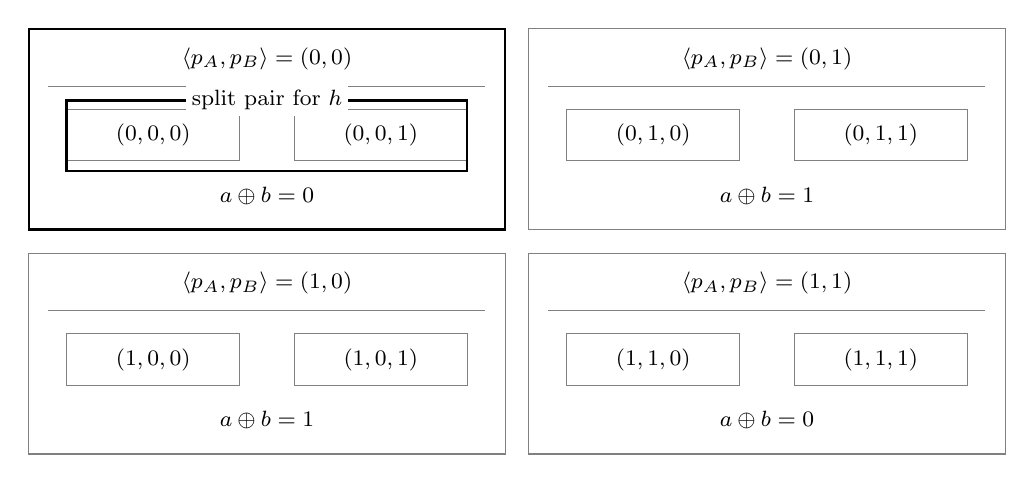
\begin{tikzpicture}[font=\footnotesize]
  \foreach \x/\y/\a/\b/\v in {
    0/0/0/0/0, 6.35/0/0/1/1,
    0/-2.85/1/0/1, 6.35/-2.85/1/1/0} {
    \draw[gray] (\x,\y) rectangle ++(6.05,-2.55);
    \node at (\x+3.025,\y-0.38)
      {$\langle p_A,p_B\rangle=(\a,\b)$};
    \draw[gray] (\x+0.25,\y-0.73) -- (\x+5.8,\y-0.73);
    \node[draw=gray,minimum width=2.2cm,minimum height=0.65cm]
      at (\x+1.58,\y-1.35) {$(\a,\b,0)$};
    \node[draw=gray,minimum width=2.2cm,minimum height=0.65cm]
      at (\x+4.47,\y-1.35) {$(\a,\b,1)$};
    \node at (\x+3.025,\y-2.12) {$a\oplus b=\v$};
  }
  \draw[black,thick] (0,0) rectangle (6.05,-2.55);
  \draw[black,thick] (0.48,-1.81) rectangle (5.57,-0.91);
  \node[fill=white,inner sep=2pt] at (3.025,-0.91) {split pair for $h$};
\end{tikzpicture}
\caption{The four fibres of $\langle p_A,p_B\rangle$ in $\{0,1\}^3$. Each contains both values of $h$ and one value of $a\oplus b$; the outlined states in the $(0,0)$ fibre form a split pair for $h$.}
\label{fig:cube}
\end{figure}


The observable $a\oplus b$ of the introduction lies between the two. It has split pairs
against each parent but none against the pairing, since $(a,b)$ determines $a\oplus b$;
it is therefore not strict. This is the elementary reason the test includes the pairing
(\Cref{sec:intro-example}).

\subsection{Refinements and cheap constructions}

\begin{definition}[Common refinement]
\label{def:common-refinement}
A map $q:J\to R$ is a \emph{common refinement} of the parents if there is
$h:R\to A\times B$ with $h\circ q=\langle p_A,p_B\rangle$.
\end{definition}

\begin{proposition}[Global factorization through the pair passes to every refinement]
\label{prop:refinement}
If $f$ factors globally through $\langle p_A,p_B\rangle$ (\Cref{def:factorization}) and $q$
is a common refinement, then $f$ factors globally through~$q$, and hence on its image.
\end{proposition}

\begin{proof}
If $f=g\circ\langle p_A,p_B\rangle$ and $h\circ q=\langle p_A,p_B\rangle$, then
$f=(g\circ h)\circ q$.
\end{proof}

\begin{remark}[The limit of strictness]
\label{rem:refinement-limit}
The converse of \Cref{prop:refinement} fails. In \Cref{ex:cube} the identity map of $J$ is
a common refinement, and the strict observable $h$ factors through it on its image.
Strictness is tested against the parents and their pairing only, and says nothing about
an arbitrary finer description of the join. A certificate that claims non-factorization
through a common refinement must therefore name that refinement and prove the claim for
it, and \Cref{thm:bridge} takes that proof as a hypothesis.
\end{remark}

The certificate language also refuses three cheap ways of manufacturing a joint
distinction: relabelling, rescheduling and coarsening. Each has a semantic counterpart.

\begin{definition}[Relabelling, scheduling and coarsening]
\label{def:cheap}
An observable $f$ of a semantic join is
\begin{enumerate}[nosep]
  \item \emph{relabelling-only} if it factors on its image through
        $\sigma\circ\langle p_A,p_B\rangle$ for some bijection $\sigma$ of $A\times B$;
  \item \emph{scheduling-only} for a declared schedule map $s:J\to S$ if it factors on its
        image through~$s$;
  \item \emph{coarsening-only} if it factors on its image through $c\circ p_A$ for some map
        $c$ out of $A$, or through $c\circ p_B$ for some map $c$ out of~$B$.
\end{enumerate}
\end{definition}

\begin{proposition}[Strictness excludes relabelling and coarsening]
\label{prop:strict-not-cheap}
A strict observable is neither relabelling-only nor coarsening-only.
\end{proposition}

\begin{proof}
A split pair for $q$ and $f$ is a split pair for $c\circ q$ and $f$, for any map $c$. The
split pairs of \Cref{thm:strict-split} for the pairing and for each parent therefore
survive composition with $\sigma$ and with $c$, and \Cref{thm:split-criterion} rules out
each factorization on the image.
\end{proof}

Scheduling is different: whether $f$ factors on its image through a schedule depends on
the schedule, and every observable factors on its image through the identity map of $J$. A schedule,
like a refinement, must therefore be declared.

\subsection{The bridge to the certificate language}
\label{sec:bridge}

The certificate language records strictness as an \emph{anti-product witness}
(\Cref{def:strict-certificate}): a record with a flag for a joint distinction, four flags
for factorization on the image through the left parent, the right parent, the declared product and the
declared common refinement, three flags for relabelling, scheduling and coarsening, a
description and an audit. The witness is valid when the first flag is set, the other seven
are clear, the description is non-empty and the audit has an entry. As a record the
witness is only an assertion. The following theorem is a soundness check: it shows that
the witness's validity predicate is satisfied by a semantic model, with every flag earned
by a proof.

\begin{theorem}[Soundness of the strictness certificate]
\label{thm:bridge}
Let $f$ be an observable of a semantic join, let $q:J\to R$ be a common refinement of the
parents, and let $s:J\to S$ be a declared schedule. Suppose $f$ is strict, does not factor
on its image through $q$, and is not scheduling-only for~$s$. Set each flag of an
anti-product witness to the truth value of its semantic counterpart: a split pair for
$\langle p_A,p_B\rangle$ and $f$; factorization on the image through $p_A$, $p_B$,
$\langle p_A,p_B\rangle$ and $q$; and the three conditions of \Cref{def:cheap}. With a
non-empty description and an audit entry, the resulting witness is valid. In particular,
\Cref{ex:cube} with $q=\langle p_A,p_B\rangle$ and $s=p_A$ yields a valid witness.
\end{theorem}

\begin{proof}
Each flag is checked against its semantic counterpart in turn.
The joint-distinction flag is set by \Cref{thm:strict-split}. The flags for the parents and
the pairing are clear because $f$ is strict, the refinement flag is clear by hypothesis,
the relabelling and coarsening flags are clear by \Cref{prop:strict-not-cheap}, and the
scheduling flag is clear by hypothesis. For the example, strictness is
\Cref{ex:cube}; the pairing is a common refinement through the identity of $A\times B$,
non-factorization through it is part of strictness, and non-factorization through $s=p_A$
is the first clause of strictness.
\end{proof}

The theorem is close to a restatement. Once strictness and the two extra hypotheses are
granted, each flag is settled in one line, by \Cref{thm:strict-split},
\Cref{prop:strict-not-cheap} or a hypothesis, and no new construction is involved. Its
role is to check the certificate language against the semantics: the Boolean witness asks
for nothing that a semantic strict join cannot supply.
The two extra hypotheses are genuine, because strictness does not supply them
(\Cref{rem:refinement-limit}).

The schedule $s=p_A$ in the example models a join assembled by running the left parent:
the schedule reads a state only through its $A$-part. It is chosen because it is the
simplest declared schedule for which the scheduling hypothesis needs no proof beyond
strictness, since non-factorization through $p_A$ is the first clause of strictness. A
schedule that sees more of $J$ than the parents do can make the hypothesis fail, as the
identity map of $J$ always does, and for such a schedule it must be proved.

The flags are truth values of propositions that need not be decidable, so the witness is
defined classically; for finite carriers \Cref{thm:split-criterion} decides them. The
theorem says nothing about the other parts of a strict-join certificate, which record
composite objecthood (that the joint candidate is a fixed point of a declared closure, an
object in the sense of Foundations~I), retention of the parents, source independence and a settled budget
(\Cref{def:strict-certificate}). Those remain recorded assertions.
